\documentclass{article}
\usepackage{tikz}
\usepackage{minted}
\usepackage{amsmath}
\usepackage{physics}
\usepackage{graphicx}
% \usepackage{xepersian}
%\usepackage{utf8}
% \settextfont{Yas}
% \setlatintextfont{Adwaita Sans}
\title{
Simulation of Reflection and Transmission by Thin Films}
\author{Bahar Ghasemzadeh\\Soroush Seirani G.}
\date{}

\begin{document}
	\maketitle
	\newpage
	
	\section*{Introduction}

	We know that electromagnetic waves refract when they encounter dielectric plates with different dielectric constants, with one part being reflected and the other part being transmitted.

	Now, if we use several thin dielectric layers, it can be said that after successive reflections and transmissions between the layers, we will ultimately have one reflected wave resulting from the interaction of an infinite number of reflected waves and one transmitted wave resulting from the interaction of an infinite number of transmitted waves.

	For the case of two semi-infinite dielectrics or just a single thin layer between them, there is an analytic solution for the reflected and transmitted energy. However, for a greater number of layers, the only approach is a numerical solution.

	In this project, by examining the fundamental relationships, we will simulate a system with an arbitrary number of thin layers using Python and investigate its applications in constructing various devices.
	
	\newpage
	
	
	\begin{center}
		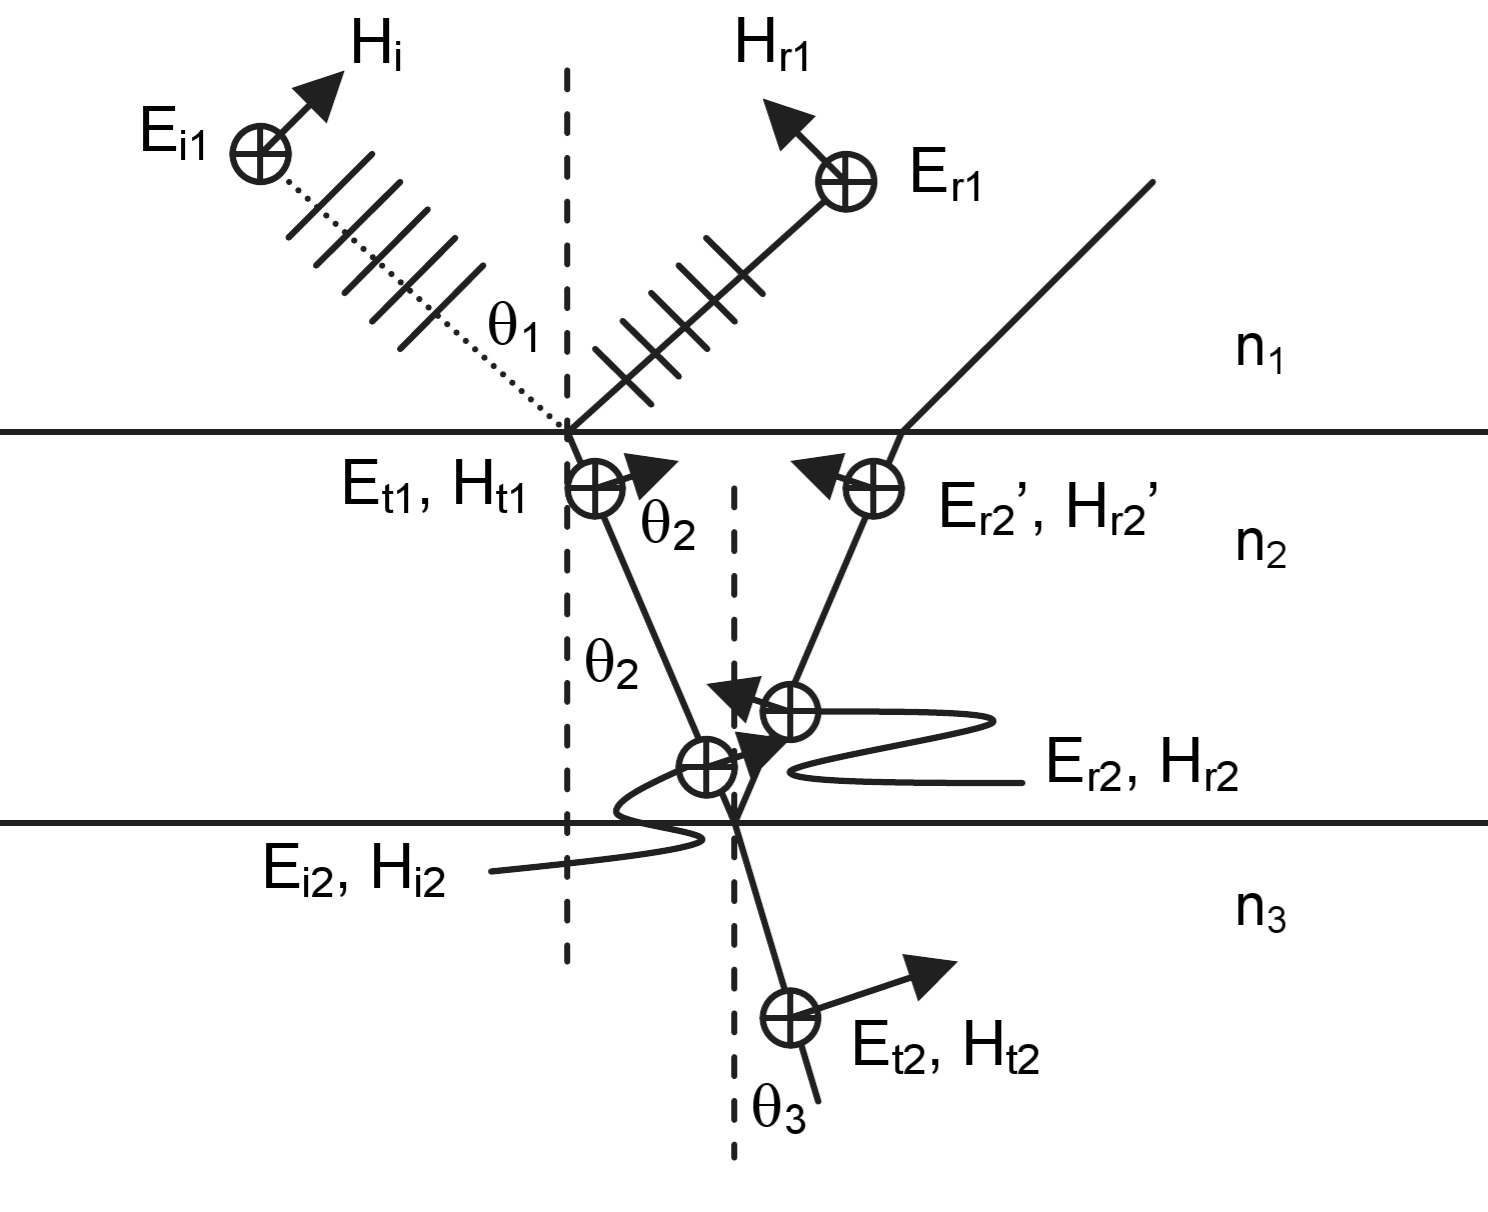
\includegraphics[height=.45\linewidth]{image2}
	\end{center}
	
	\section*{Examining Relationships and Boundary Conditions}
	
	To examine the relationships, we consider the direction perpendicular to the layers as $z$ and also take the $\mathbf{k}$ vector plane to be the $x$-$z$ plane.

	To simplify calculations, we consider $s$-polarization in the $y$ direction, and thus $p$-polarization will be in the $x$-$z$ plane.
	
	
	
	
	\subsection*{$s$-Polarization at the boundary of media $i$ and $i+1$:}
	
	\begin{gather*}
		n_i \sin \theta_i= n _{i+1} \sin \theta_{i+1}\\
		E_i+E_{ir}=E_{it}\\
		n_i \cos \theta_i(	E_i-E_{ir})=n_{i+1}\cos \theta_{i+1} E_{it}\\
		\Rightarrow r^s_{i,i+1}=\frac{E_{ir}}{E_i}=\frac{B_{ir}}{B_i}=\frac{n_i \cos \theta_i-n_{i+1}\cos \theta_{i+1}}{n_i \cos \theta_i+n_{i+1}\cos \theta_{i+1}}\\
		\Rightarrow t^s_{i,i+1}=\frac{E_{it}}{E_i}=\frac{n_{i+1} B_{it}}{n_i B_i}=\frac{2n_i \cos \theta_i}{n_i \cos \theta_i+n_{i+1}\cos \theta_{i+1}}\\
		R^s=\frac{|\mathbf{E_{r}}\cross \mathbf{B_{r}}|}{|\mathbf{E}\cross \mathbf{B}|}=r^s r^{s*}\\
		T^s=\frac{|\mathbf{E_{t}}\cross \mathbf{B_{t}}|\cos \theta_{N}}{|\mathbf{E}\cross \mathbf{B}|\cos \theta_1}=\frac{n_N\cos \theta_N}{n_1\cos \theta_1} t^s t^{s*}
	\end{gather*}
	
	In these equations, the coefficients $r,t$ are obtained from the interaction of the reflected and transmitted waves, which for the case of no thin film or one thin film has an analytic solution, but otherwise requires a numerical solution.
	
	\newpage
	\subsection*{$p$-Polarization at the boundary of media $i$ and $i+1$:}
	
	\begin{gather*}
		n_i \sin \theta_i= n _{i+1} \sin \theta_{i+1}\\
		n_i(E_i+E_{ir})=n_{i+1}E_{it}\\
		\cos \theta_i(	E_i-E_{ir})=\cos \theta_{i+1} E_{it}\\
		\Rightarrow r^p_{i,i+1}=\frac{E_{ir}}{E_i}=\frac{B_{ir}}{B_i}=\frac{n_{i+1}\cos\theta_i-n_i \cos \theta_{i+1}}{n_i \cos \theta_{i+1}+n_{i+1}\cos \theta_i}\\
		\Rightarrow t^p_{i,i+1}=\frac{E_{it}}{E_i}=\frac{n_{i+1} B_{it}}{n_i B_i}=\frac{2n_i \cos \theta_i}{n_i \cos \theta_{i+1}+n_{i+1}\cos \theta_i}\\
		R^p=\frac{|\mathbf{E_{r}}\cross \mathbf{B_{r}}|}{|\mathbf{E}\cross \mathbf{B}|}=r^p r^{p*}\\
		T^p=\frac{|\mathbf{E_{t}}\cross \mathbf{B_{t}}|\cos \theta_{N}}{|\mathbf{E}\cross \mathbf{B}|\cos \theta_1}=\frac{n_N\cos \theta_N}{n_1\cos \theta_1} t^p t^{p*}
	\end{gather*}
	
	Similar to the previous equation, the coefficients $r,t$ are obtained from the interaction of the reflected and transmitted waves, which for the case of no thin film or one thin film has a parametric solution, but otherwise requires a numerical solution.
	\\
	Furthermore, to calculate the interactions, it is necessary to know the phase difference after traversing the length of each layer:
	\begin{gather*}
		\beta_i=d_ik_i\cos\theta_i=\frac{2\pi}{\lambda_i}d_i\cos\theta_i
	\end{gather*}
	
	\begin{center}
		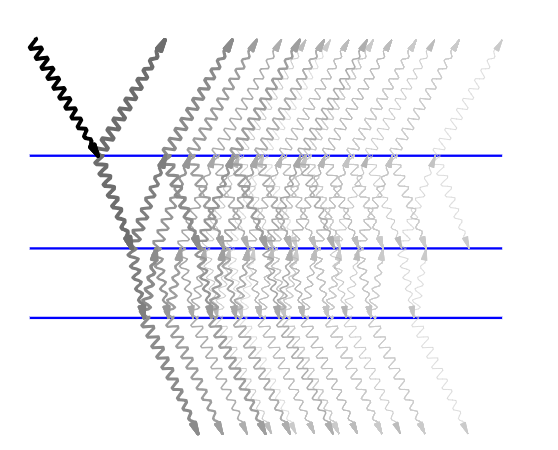
\includegraphics[height=.45\linewidth]{wAN1K}
	\end{center}
	\newpage	

	
	\section*{Applications of Electromagnetic Wave Interference in Thin Films}
	\subsection*{1. Anti-Reflection Coatings}
	
	
	Here, by using destructive interference of the reflected waves, we reduce the reflection from the object's surface. Applications of this include anti-glare glasses, smartphone and display screens, and increasing light absorption in solar cells.
    
	Now, let's examine an example of materials that are practically used for making anti-glare glasses:
	
	In this example, the reflection coefficient becomes zero in the visible light range due to destructive interference in the layers.
	
	\begin{center}
		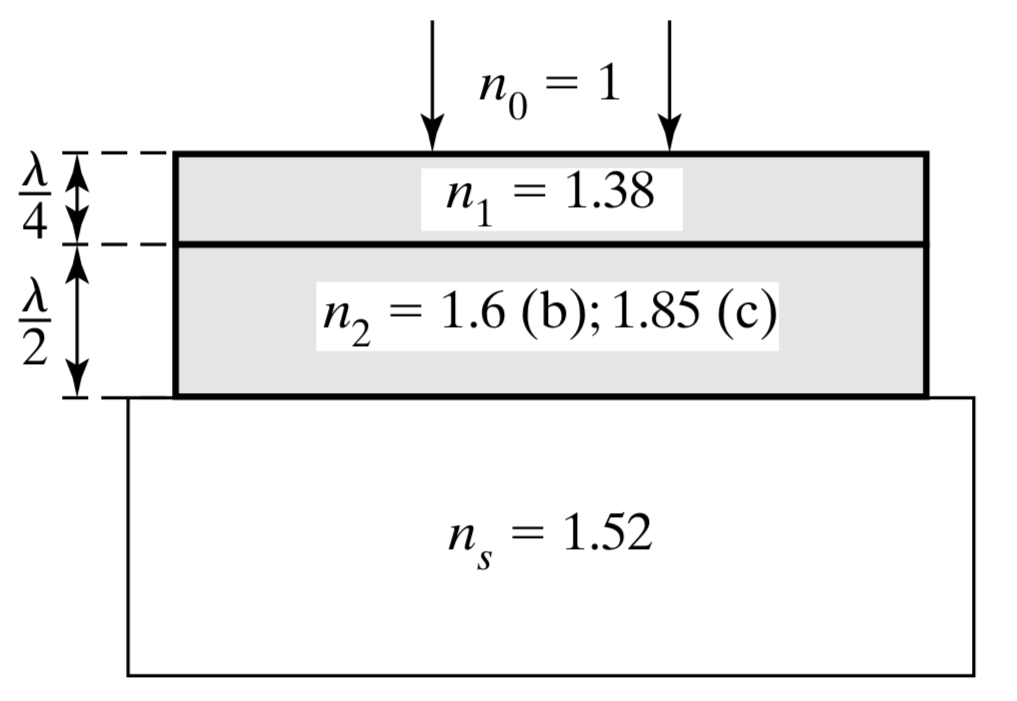
\includegraphics[height=.3\linewidth]{image_2025-07-16_20-45-14}
	\end{center}
	In the optics book by Pedrotti, this system is examined for visible wavelengths at normal incidence to the surface, and the resulting graph is as follows:
	\begin{center}
		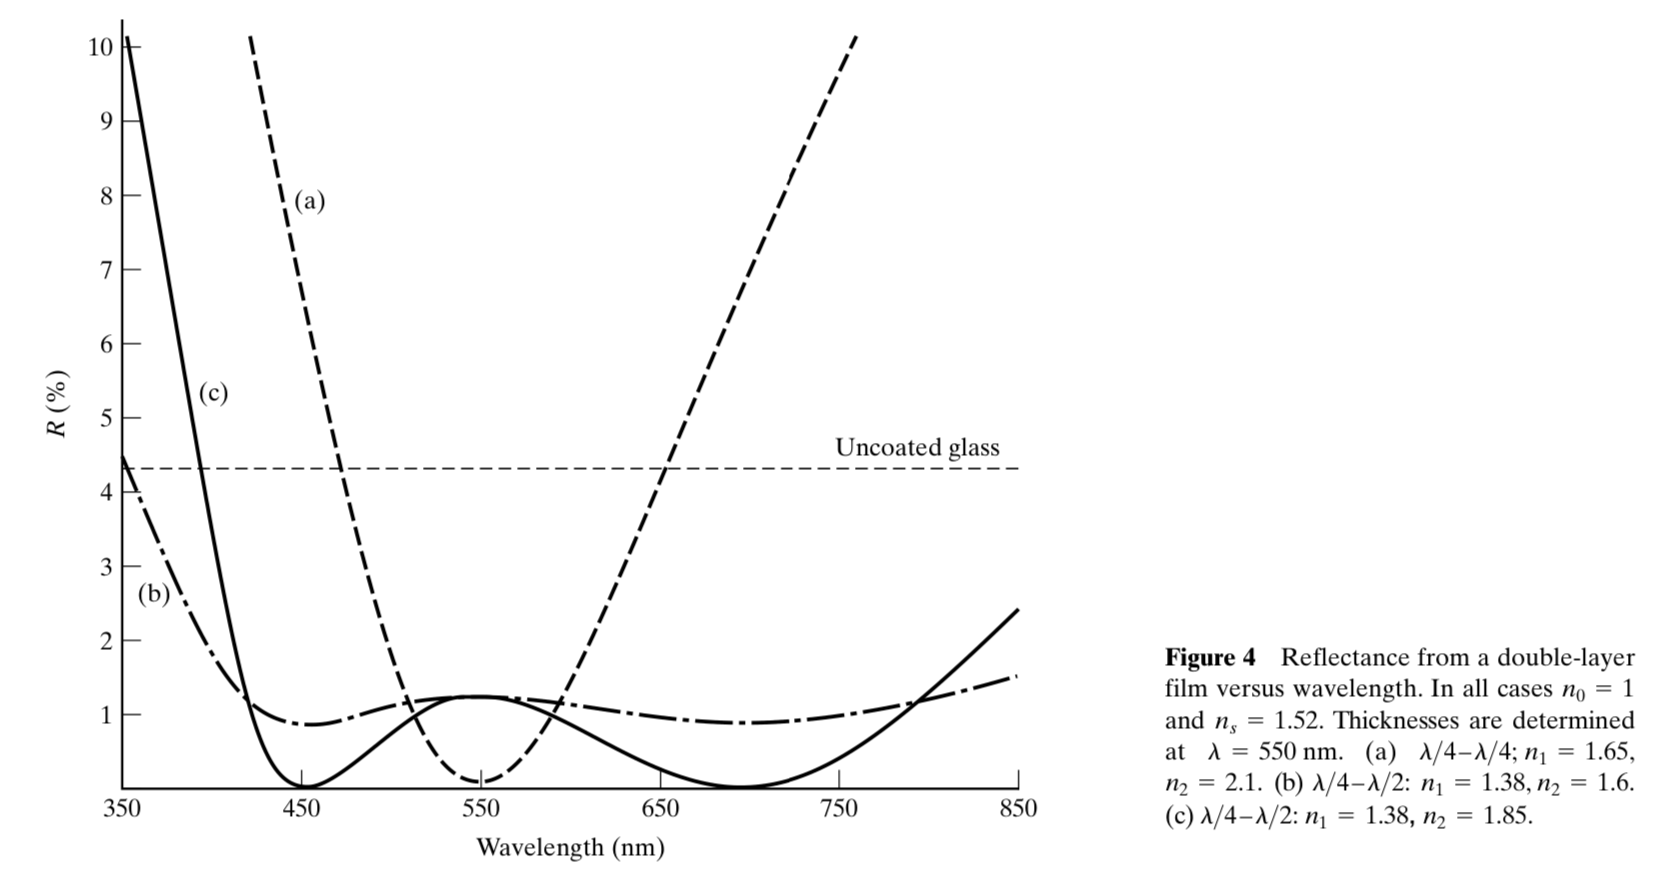
\includegraphics[height=.5\linewidth]{image_2025-07-16_20-39-13}
	\end{center}
	\newpage
	It can also be observed that in this example, the simulation code yields identical results.
	\begin{center}
		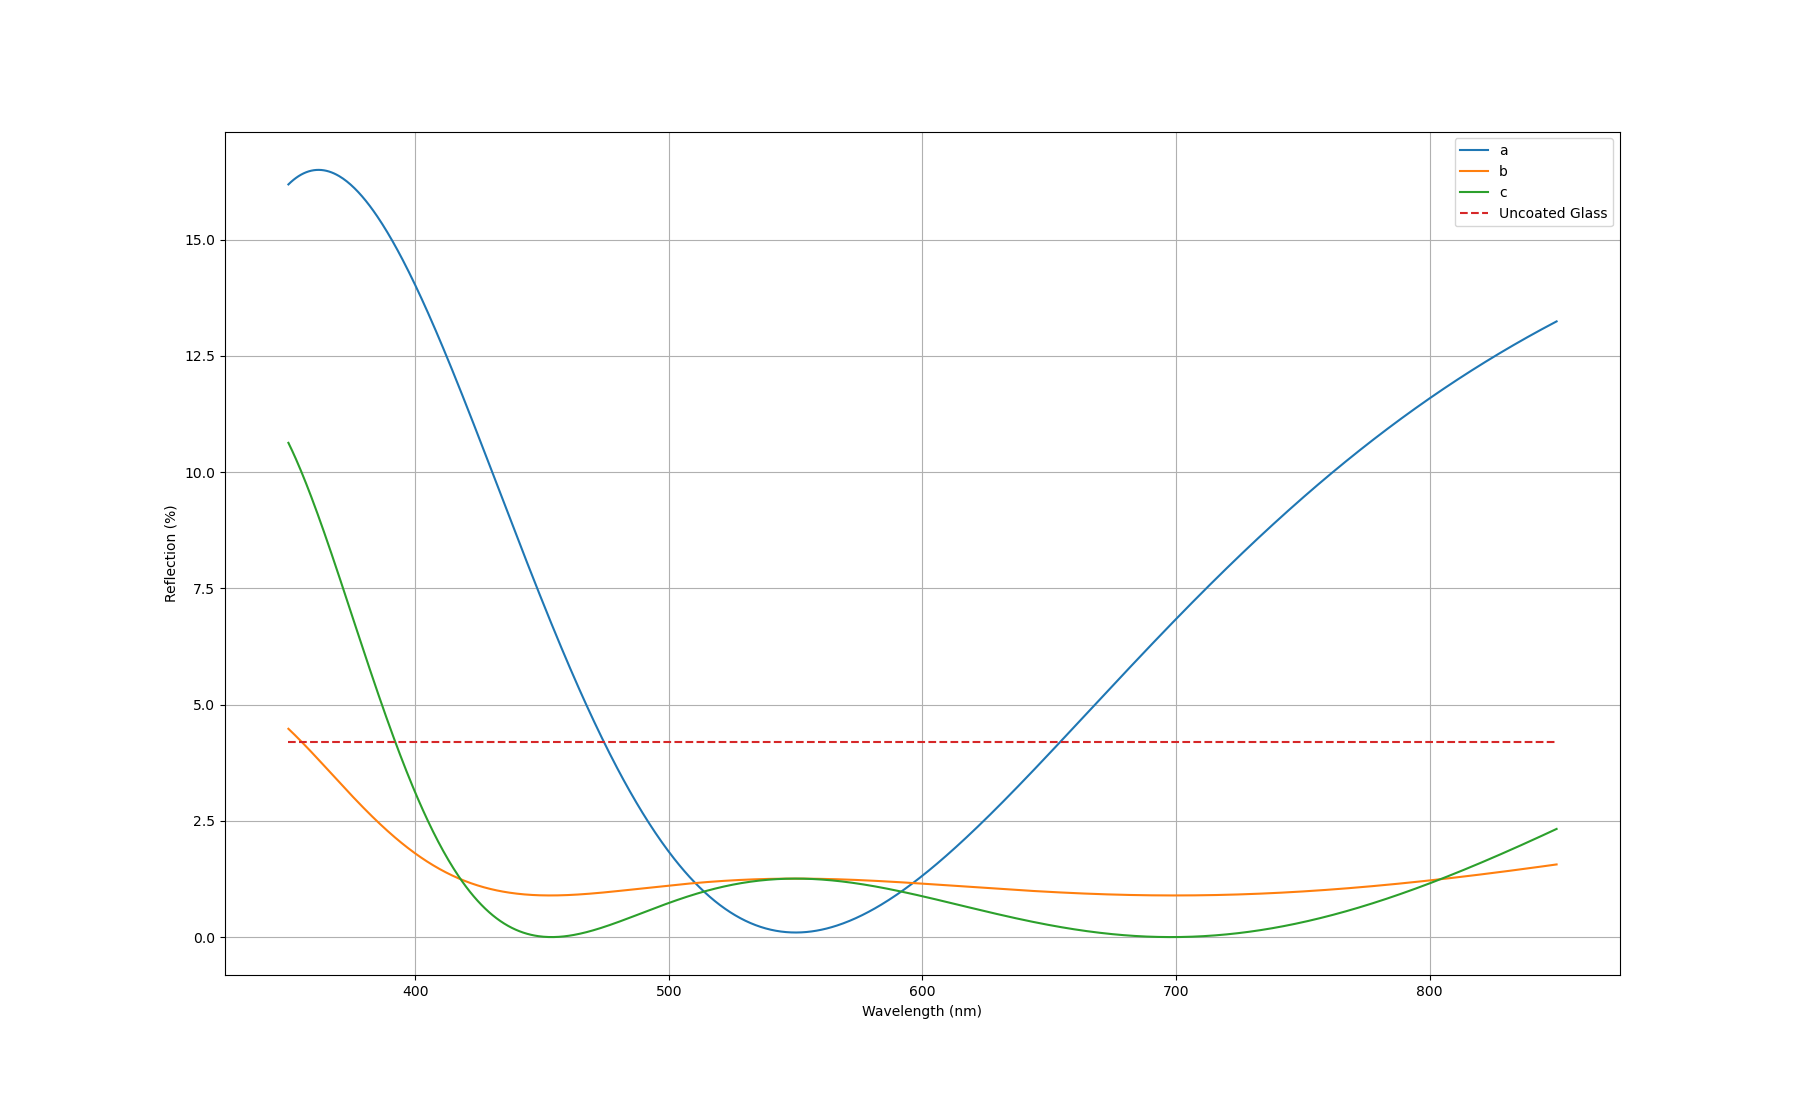
\includegraphics[height=.5\linewidth]{fig1}
	\end{center}
	
	\subsection*{2. Lasers}
	
	
	As a final application, thin dielectric layers are used as internal coatings for laser cavities.
	
	These layers create constructive interference at a specific frequency, which causes resonance at our desired frequency, and the reflection at that frequency will reach its highest possible value.
	\newpage
	
	
	
	\section*{Algorithm Workflow}
		
		This algorithm calculates the reflection from thin films by simulating light propagation as the superposition of waves that are reflected and transmitted multiple times at the boundaries. This algorithm has several important parts, which are explained below.
		
	\subsection*{Wave Splitting}
		
		At each boundary, the incident wave splits into a reflected wave and a transmitted wave. Using the Fresnel equations, the intensity of both waves is calculated, and the effectiveness of the incident wave ends here.
		
	\subsection*{Phase Summation}
		
		Waves develop a phase difference relative to each other due to the different paths they travel. This algorithm calculates and applies the phase changes of the waves by considering the wavelength, the refractive index of the medium, and the angle of propagation.
		
	\subsection*{Interference}
		
		Finally, by superimposing all the reflected waves and considering their intensity and phase difference with each other, the reflection coefficient can be calculated.
		
	\subsection*{Simulation Termination}
		
		Whenever the intensity of a ray becomes negligible, it is removed from the simulation. The simulation continues until all rays have either exited the layer or become too weak to be significant ($10^{-6}$ times the intensity of the initial ray).
		
	\section*{Program Usage Guide}
		
		To run the program, you need the Python libraries numpy and matplotlib. The main program file is named thinfilms.py. There is also another file called glasses.py which calculates the reflection from a series of pre-defined layers and displays it on a graph.
		
		After running the main file, a series of questions will be asked, which you must answer as shown in the figure below:
		
	\begin{center}
		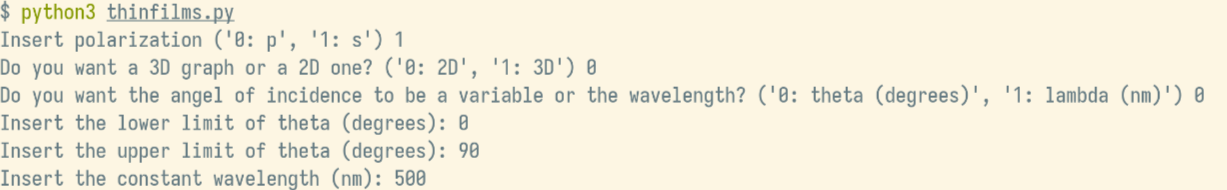
\includegraphics[height=0.15\linewidth]{questions.png}
	\end{center}
		
		After answering all the questions, wait for the calculations to finish and the graph to be displayed.
		
		To change the layers used in the simulation, you can modify the films variable similar to the example below:
		
	% \begin{latin}
		\begin{minted}{python}
            films = [[1,     0],     # First layer n_0
                    [2.25,  300],
                     ...
                    [k (Dielectric Constant), d (Film Thickness)],
                    ...
                    [2.3104, 0]]   # Last layer  n_s            
		\end{minted}
	% \end{latin}
	
	
	
	
	
	
	
	
	
\end{document}
